\documentclass[12pt]{article}
\usepackage[spanish,es-nodecimaldot]{babel}
\usepackage[utf8]{inputenc}
\usepackage[T1]{fontenc}
\usepackage[a4paper,margin=2.5cm]{geometry}
\usepackage{lmodern}
\usepackage{setspace}
\usepackage{parskip}
\usepackage{graphicx}
\usepackage{float}
\usepackage{amsmath}

\begin{document}
\thispagestyle{empty}

\begin{center}
    \textsc{Universidad Central de Venezuela}\\[0.35cm]
    \textsc{Facultad de Ingenier\'ia}\\[0.35cm]
    \textsc{Escuela de Ingenier\'ia El\'ectrica}\\[0.35cm]
    \textsc{Departamento de Potencia}\\[0.35cm]
    \textsc{Laboratorio de M\'aquinas El\'ectricas I}
\end{center}

\vspace{6.8cm}

\begin{center}
    \textbf{PRE-LABORATORIO N\textsuperscript{o} 7}\\[0.35cm]
    \textbf{Transformador monof\'asico en Paralelo}
\end{center}

\vfill

\noindent
\begin{minipage}[t]{0.48\textwidth}
    Docente:\\[0.25cm]
    Jes\'us Blondel
\end{minipage}%
\hfill
\begin{minipage}[t]{0.48\textwidth}
    \raggedleft
    Autor:\\[0.25cm]
    Br. Carla Fajardo\\[0.25cm]
    V-27.571.576
\end{minipage}

\vspace{1.1cm}

\begin{center}
    Caracas, \today
\end{center}

\newpage

\section{Introducci\'on}

La conexi\'on de transformadores monof\'asicos en paralelo permite aumentar la capacidad de suministro y brindar mayor flexibilidad operativa ante cambios en la demanda, por lo que esta configuraci\'on es muy utilizada en sistemas de potencia. Tambi\'en facilita las labores de mantenimiento, ya que es posible retirar una unidad de servicio mientras las restantes contin\'uan alimentando la carga. Para operar de forma segura, los transformadores deben conectarse con polaridades compatibles y tensiones secundarias adecuadas.

Por lo tanto, antes de acoplar los secundarios es necesario verificar la polaridad y caracterizar el comportamiento de cada transformador. El an\'alisis de estas condiciones permite anticipar posibles sobrecargas y p\'erdidas adicionales.

En este prelaboratorio se estudia la operaci\'on en paralelo de dos transformadores monof\'asicos. Se determinan te\'oricamente la diferencia entre las tensiones secundarias y la corriente circulatoria, y se plantea la verificaci\'on experimental de las condiciones de conexi\'on. Asimismo, se considera el comportamiento del banco en vac\'io y bajo carga resistiva mediante el registro de tensiones, corrientes y potencias, con el fin de analizar el reparto de carga entre los transformadores.

\newpage

\section{Objetivos}

\subsection*{Objetivo general}
Analizar la conexi\'on y el comportamiento de dos transformadores monof\'asicos operando en paralelo, tanto en vac\'io como bajo carga resistiva.

\subsection*{Objetivos espec\'ificos}
\begin{itemize}
    \item Verificar las condiciones necesarias para conectar los transformadores en paralelo, incluyendo la polaridad, la relaci\'on de transformaci\'on y la impedancia de cortocircuito.
    \item Determinar te\'oricamente la diferencia entre las tensiones secundarias y la corriente circulatoria en vac\'io.
    \item Medir las tensiones y corrientes del banco en paralelo en vac\'io y bajo distintos niveles de carga resistiva.
    \item Analizar el reparto de corriente y potencia entre los transformadores a partir de las mediciones experimentales.
\end{itemize}
\newpage

\section{Marco te\'orico}

\subsection{Conexi\'on de transformadores en paralelo}

Dos o m\'as transformadores operan en paralelo cuando sus bornes hom\'ologos se conectan entre s\'i en los devanados primarios y secundarios. Los devanados primarios se conectan a las mismas barras de alimentaci\'on, mientras que los secundarios se conectan a barras comunes que suministran energ\'ia a la carga. En la pr\'actica, las conexiones se realizan mediante conductores cuya impedancia es despreciable frente a la de los transformadores.

\subsubsection{Ventajas operativas principales}
\begin{itemize}
    \item \textbf{Flexibilidad y ampliaci\'on:} permite incrementar la capacidad instalada de una subestaci\'on para atender aumentos de demanda sin reemplazar el transformador existente.
    \item \textbf{Optimizaci\'on del rendimiento:} en periodos de baja demanda es posible desconectar una o m\'as unidades para que las restantes operen cerca de su punto de rendimiento m\'aximo, evitando mantener un transformador grande a baja carga.
    \item \textbf{Confiabilidad del suministro:} facilita el mantenimiento preventivo o la reparaci\'on de aver\'ias sin interrumpir por completo el suministro el\'ectrico a las cargas esenciales.
\end{itemize}

\subsection{Condiciones para la conexi\'on en paralelo}

Para lograr un acoplamiento seguro y un reparto adecuado de la carga, se deben considerar las siguientes condiciones:
\begin{enumerate}
    \item \textbf{Igualdad de las relaciones de transformaci\'on:} es una condici\'on obligatoria tanto en vac\'io como bajo carga. Una diferencia entre las tensiones secundarias puede provocar corrientes circulatorias.
    \item \textbf{Misma polaridad y desfase nulo:} los transformadores deben tener la misma polaridad y pertenecer al mismo grupo de conexi\'on, de modo que sus tensiones secundarias est\'en en fase.
    \item \textbf{Igualdad de las tensiones relativas de cortocircuito:} es deseable para que la carga se reparta de manera proporcional a las potencias nominales de las unidades.
\end{enumerate}

En la pr\'actica pueden admitirse diferencias limitadas entre las tensiones de cortocircuito; como criterio orientativo, se recomienda que no excedan el 10\%. Tambi\'en se recomienda que la relaci\'on entre las potencias nominales de los transformadores conectados no supere 3:1, para evitar desequilibrios t\'ermicos importantes.

\subsection{Corriente circulatoria}

Si se conectan en paralelo transformadores cuyas relaciones de transformaci\'on no son id\'enticas o cuyas tensiones secundarias presentan un desfase angular, aparece una diferencia de potencial entre sus secundarios incluso cuando funcionan en vac\'io ($I_{\mathrm{carga}}=0$). Esta diferencia origina una corriente interna que circula en un lazo cerrado entre los devanados secundarios:
\begin{equation}
    I_{\mathrm{c}} = \frac{E_{2\mathrm{I}}-E_{2\mathrm{II}}}{Z'_{\mathrm{ccI}}+Z'_{\mathrm{ccII}}}
\end{equation}
Aqu\'i, $E_{2\mathrm{I}}$ y $E_{2\mathrm{II}}$ son las fuerzas electromotrices secundarias en vac\'io, y $Z'_{\mathrm{ccI}}$ y $Z'_{\mathrm{ccII}}$ son las impedancias de cortocircuito de cada transformador referidas al secundario.

\subsubsection{Efectos de la corriente circulatoria}
\begin{enumerate}
    \item \textbf{Calentamiento e incremento de p\'erdidas:} aumenta las p\'erdidas por efecto Joule ($I_{\mathrm{c}}^2R_{\mathrm{cc}}$) sin realizar trabajo hacia la carga externa.
    \item \textbf{Reducci\'on de la capacidad disponible:} la corriente circulatoria consume parte de la capacidad de corriente de los devanados y reduce la potencia efectiva utilizable por la instalaci\'on.
    \item \textbf{Riesgo de sobrecarga en vac\'io:} si la diferencia entre las relaciones de transformaci\'on o el desfase es considerable, la corriente circulatoria puede acercarse a la corriente nominal y sobrecalentar los transformadores aun sin carga conectada.
\end{enumerate}

\subsection{Reparto de cargas}

Cuando dos transformadores en paralelo alimentan una carga com\'un, ambos quedan sometidos a la misma tensi\'on primaria y a la misma tensi\'on secundaria. Por lo tanto, las ca\'idas de tensi\'on internas en sus impedancias de cortocircuito son iguales:
\begin{equation}
    \Delta V_{\mathrm{I}}=\Delta V_{\mathrm{II}}
    \quad\Longrightarrow\quad
    I_{\mathrm{I}}Z_{\mathrm{ccI}}=I_{\mathrm{II}}Z_{\mathrm{ccII}}
\end{equation}

\subsubsection{Reparto seg\'un el \'indice de carga}
El \'indice de carga se define como $C=I/I_N$. La tensi\'on relativa de cortocircuito se expresa como:
\begin{equation}
    \varepsilon_{\mathrm{cc}}=\frac{I_N Z_{\mathrm{cc}}}{V_N}\times 100\%
\end{equation}
La relaci\'on entre los \'indices de carga de las dos unidades es inversamente proporcional a sus tensiones relativas de cortocircuito:
\begin{equation}
    \frac{C_{\mathrm{I}}}{C_{\mathrm{II}}}
    =\frac{\varepsilon_{\mathrm{ccII}}}{\varepsilon_{\mathrm{ccI}}}
\end{equation}

\begin{itemize}
    \item \textbf{Tensiones relativas de cortocircuito iguales:} los \'indices de carga son iguales y la carga total se distribuye en proporci\'on a las potencias nominales:
    \begin{equation}
        S_{\mathrm{I}}=S_T\left(\frac{S_{N\mathrm{I}}}{S_{N\mathrm{I}}+S_{N\mathrm{II}}}\right),
        \qquad
        S_{\mathrm{II}}=S_T\left(\frac{S_{N\mathrm{II}}}{S_{N\mathrm{I}}+S_{N\mathrm{II}}}\right)
    \end{equation}
    \item \textbf{Tensiones relativas de cortocircuito distintas:} el transformador con menor tensi\'on relativa de cortocircuito asumir\'a un \'indice de carga mayor, por lo que puede alcanzar su capacidad nominal o sobrecargarse antes que la otra unidad.
\end{itemize}

\subsubsection{Reparto en funci\'on de las impedancias complejas}
Para transformadores con impedancias de cortocircuito complejas, la potencia aparente aportada por cada unidad se puede expresar como:
\begin{equation}
    S_{\mathrm{I}}=S_T\left(\frac{Z'_{\mathrm{ccII}}}{Z'_{\mathrm{ccI}}+Z'_{\mathrm{ccII}}}\right),
    \qquad
    S_{\mathrm{II}}=S_T\left(\frac{Z'_{\mathrm{ccI}}}{Z'_{\mathrm{ccI}}+Z'_{\mathrm{ccII}}}\right)
\end{equation}
\newpage

\section{Trabajo previo}

\subsection{Par\'ametros para los c\'alculos}

De acuerdo al transformador utilizado en las pr\'acticas anteriores:
Transformador a:
\begin{itemize}
    \item $S_n = 2\,\text{kVA}$
    \item $V_n = 120/240\,\text{V}$
    \item $a_{Ta} = 2{,}29$
    \item $Z_{cca} = 1{,}38\angle 24{,}47^\circ\,\Omega$
\end{itemize}

Transformador b:
\begin{itemize}
    \item $S_n = 2\,\text{kVA}$
    \item $V_n = 120/240\,\text{V}$
    \item $a_{Tb} = 2{,}40$ (se asume 0{,}5$\%$ mayor que $a_{Ta}$)
    \item $Z_{ccb} = 1{,}45\angle 14{,}055^\circ\,\Omega$ (se asume 0{,}5$\%$ mayor que $Z_{cca}$)
\end{itemize}

\subsection{Corriente circulatoria}

Con una tensi\'on de alimentaci\'on de $U_1 = 120\,\text{V}$ en el primario, las tensiones en el secundario se calculan de la siguiente manera:

\begin{equation}
    E_{a2} = \frac{U_1}{a_{Ta}}
\end{equation}

\begin{equation}
    E_{b2} = \frac{U_1}{a_{Tb}}
\end{equation}

Entonces, la diferencia de potencial entre los secundarios, con SW1 y SW2 abiertos, es:
\begin{equation}
    \Delta E_{a2} = \frac{U_1}{a_{Ta}} - \frac{U_1}{a_{Tb}}
\end{equation}

Sustituyendo los valores correspondientes:
\[
    \Delta E_{a2} = \frac{120}{2{,}29} - \frac{120}{2{,}40} 
\]
$\Delta E_{a2} = 2{,}40\,\text{V}$.

Cuando las tensiones inducidas son diferentes, aparece una corriente circulatoria que, bajo condición de vacío, viene dada por:
\begin{equation}
    I_{a2} = -I_{b2} = \frac{\Delta E_{a2}}{Z_{cca} + Z_{ccb}}
\end{equation}

Sustituyendo los valores se tiene:
\[
    I_{a2} = \frac{2{,}40\angle 0^\circ}{(1{,}38\angle 24{,}47^\circ) + (1{,}45\angle 14{,}055^\circ)}
\]
Por lo tanto, $I_{a2} = 0{,}851\angle -19{,}133^\circ\,\text{A}$.

\newpage

\section{Equipos e instrumentos}
\begin{table}[H]
\centering
\begin{tabular}{|c|}
\hline
\textbf{Equipo/Instrumento} \\ \hline
Transformador monof\'asico \\ \hline
Variac (Autotransformador variable) \\ \hline
Volt\'imetro de hierro m\'ovil \\ \hline
Amper\'imetro de hierro m\'ovil \\ \hline
Vat\'imetro \\ \hline
Fuente de alimentaci\'on AC \\ \hline
Carga \\ \hline
Cables de conexi\'on \\ \hline
Interruptor de prueba \\ \hline
\end{tabular}
\end{table}

\newpage

\section{Diagramas de conexi\'on}

\begin{figure}[H]
    \centering
    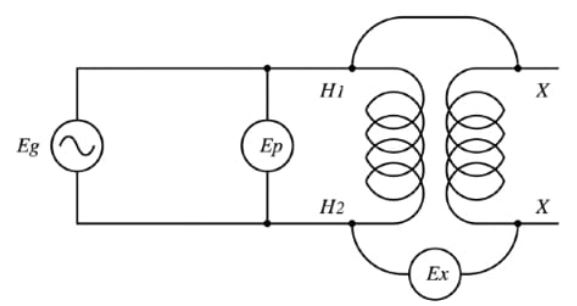
\includegraphics[width=0.7\textwidth]{imagenes/polaridad.JPG}
    \caption{Prueba de polaridad del transformador monof\'asico.}
    \label{fig:polaridad-transformador}
\end{figure}

\begin{figure}[H]
    \centering
    \includegraphics[width=0.9\textwidth]{imagenes/pueba\space de\space cortocircuito.JPG}
    \caption{Prueba de cortocircuito del transformador monof\'asico.}
    \label{fig:cortocircuito-transformador}
\end{figure}

\begin{figure}[H]
    \centering
    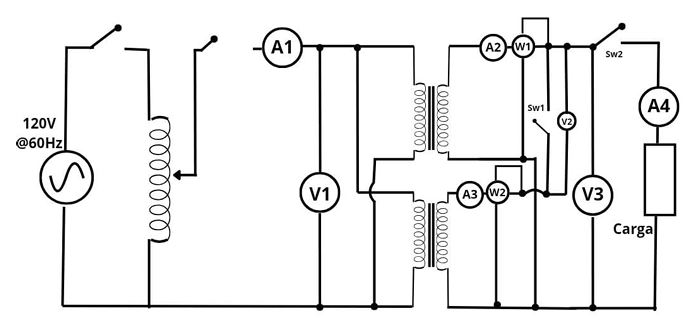
\includegraphics[width=0.9\textwidth]{imagenes/tx_paralelos.JPG}
    \caption{Transformadores monof\'asicos conectados en paralelo.}
    \label{fig:transformadores-paralelo}
\end{figure}

\section{Metodolog\'ia}

Para poder relizar el experimento, se deben seguir los siguientes pasos:

\subsection{Verificaci\'on de las condiciones para poder conectar los transformadores en paralelo}
\begin{enumerate}
    \item Seleccionar dos transformadores monof\'asicos con la misma tensi\'on de placa, prefer\'iblemente de diferentes fabricantes.
    \item Luego realizar los ensayos correspondientes paradeterminar la polaridad y la impedancia en cortocircuito del transformador a\'un no caracterizado y registrar los valores obtenidos.
    \item Se debe asegurar la polaridad identica y la coincidencia de fase y magnitud de las tensiones del secundario. Esto debe realizarse antes de establecer la conexi\'on en paralelo de los transformadores.
\end{enumerate}

\subsection{Conexi\'on de los transformadores en paralelo}
\begin{enumerate}
    \item Conectar los devanados primarios de ambos transformadores en paralelo al Variac.
    \item Conectar los devanados secundarios en paralelo, asegurando que los terminales de igual polaridad est\'en unidos. 
    \item Conectar el conjunto de secundarios a un banco de carga variable.
\end{enumerate}

\subsection{Mediciones}

\subsubsection{Sin Carga}

\begin{enumerate}
    \item Energizar los transformadores a su tensi\'on nominal.
    \item Tomar los valores de tensi\'on del primario y el secundario
    \item Medir la corriente circulatoria en el secundario de cada transformador.
\end{enumerate}

\subsubsection{Carga Variable}

\begin{enumerate}
    \item Colocar una carga a los transformadores conetados en paralelo y variar gradualmente la carga desde vac\'io hasta la capacidad nominal combinada.
    \item Para cada punto registrar los valores de tensi\'on primaria y secundaria, corriente total de carga y las corrientes individualesde cada transformador, adem\'as de registrar las potencias entregadas por cada unidad.
\end{enumerate}

\section{Tabla de Resultados}

\renewcommand{\tablename}{Cuadro}
\setcounter{table}{1}

\begin{table}[H]
\centering
\small
\renewcommand{\arraystretch}{1.15}
\caption{Caracterizaci\'on del transformador auxiliar ($T_b$): polaridad y ensayo de cortocircuito.}
\begin{tabular}{|p{0.43\textwidth}|c|p{0.28\textwidth}|c|}
\hline
\textbf{Par\'ametro} & \textbf{S\'imbolo} & \textbf{Valor medido} & \textbf{Unidad} \\ \hline
Tensi\'on de alimentaci\'on reducida de prueba & $V_{\mathrm{alim}}$ & & V \\ \hline
Tensi\'on entre terminales libres ($H_2$--$X_2$) & $V_{\mathrm{med}}$ & & V \\ \hline
Polaridad verificada ($V_{\mathrm{med}} < V_{\mathrm{alim}} \Rightarrow$ sustractiva) & -- & & -- \\ \hline
Corriente primaria de cortocircuito & $I_{ccb}$ & & A \\ \hline
Tensi\'on primaria de cortocircuito & $V_{ccb}$ & & V \\ \hline
Potencia activa de cortocircuito & $P_{ccb}$ & & W \\ \hline
Resistencia equivalente referida al secundario & $R'_{ccb}$ & & $\Omega$ \\ \hline
Reactancia equivalente referida al secundario & $X'_{ccb}$ & & $\Omega$ \\ \hline
Impedancia de cortocircuito en por unidad & $z_{ccb,\mathrm{pu}}$ & & pu \\ \hline
\end{tabular}
\end{table}


\begin{table}[H]
\centering
\small
\renewcommand{\arraystretch}{1.2}
\caption{Registro experimental sin carga conectada}
\resizebox{\textwidth}{!}{%
\begin{tabular}{|c|c|c|c|c|c|c|}
\hline
$U_1$ (V) & $I_{a1}$ (A) & $I_{b1}$ (A) & $I_{1,\mathrm{tot}}$ (A) & $V_2$ (V) & $I_{\mathrm{circ,med}}$ (A) & $P_0$ (W) \\ \hline
\rule{0pt}{0.55cm} & & & & & & \\ \hline
\rule{0pt}{0.55cm} & & & & & & \\ \hline
\end{tabular}%
}
\end{table}

\begin{table}[H]
\centering
\small
\renewcommand{\arraystretch}{1.2}
\caption{Registro experimental del banco en paralelo bajo carga resistiva}
\resizebox{\textwidth}{!}{%
\begin{tabular}{|c|c|c|c|c|c|c|c|c|}
\hline
\textbf{Punto} & $U_1$ (V) & $I_{1a,\mathrm{tot}}$ (A) & $V_2$ (V) & $I_{a2}$ (A) & $I_{b2}$ (A) & $I_L$ (A) & $P_a$ (W) & $P_b$ (W) \\ \hline
\rule{0pt}{0.55cm} & & & & & & & & \\ \hline
\rule{0pt}{0.55cm} & & & & & & & & \\ \hline
\rule{0pt}{0.55cm} & & & & & & & & \\ \hline
\rule{0pt}{0.55cm} & & & & & & & & \\ \hline
\rule{0pt}{0.55cm} & & & & & & & & \\ \hline
\end{tabular}%
}
\end{table}
\newpage

\section{Referencias}
\begin{enumerate}
    \item Nerio Ojeda, Juli\'an P\'erez. \textit{Pr\'actica 6. Transformador Monof\'asico. Rendimiento}. Universidad Central de Venezuela, Facultad de Ingenier\'ia, Escuela de Ingenier\'ia El\'ectrica, Departamento de Potencia, Laboratorio de M\'aquinas I, Revisi\'on 2012.
    \item Fraile Mora, Jes\'us. \textit{M\'aquinas El\'ectricas} (6.\textsuperscript{a} ed.). McGraw-Hill, 2008.
    \item Fitzgerald, A. E., Kingsley, C., Umans, S. D. \textit{M\'aquinas El\'ectricas}. McGraw-Hill, 6.\textsuperscript{a} ed., 2003.
    \item Chapman, S. J. \textit{M\'aquinas El\'ectricas}. McGraw-Hill, 5.\textsuperscript{a} ed., 2012.
\end{enumerate}

\end{document}
